% -*- root: Dissertation.tex -*-
\documentclass[Dissertation.tex]{subfiles}
\begin{document}
\graphicspath{{../Figures/}}
\chapter{Space-Time DPG for Compressible Navier-Stokes}
\label{sec:compressible}

% \section{Introduction}
DPG for steady compressible Navier-Stokes was studied by Jesse Chan in \cite{JesseDissertation}.
He observed that a pseudo-time stepping technique was necessary to get the Gauss-Newton solve to converge 
to a quality solution.
This suggested that space-time approach which naturally includes the transient terms
might achieve such results with a simpler Newton iteration.

We derive an ultra-weak space-time divergence formulation of the transient compressible Navier-Stokes equations,
linearizing and developing robust test norms in a similar manner as was done in the previous chapter.
We focus our numerical results on shock tube problems for which analytical solutions are known for the 
inviscid Euler equations.
Despite the absence of any sophisticated shock capturing, we are able to resolve the shocks with adaptivity 
and produce some decent numerical results.

\section{Nonlinear Form}

The compressible Navier-Stokes equations are
\begin{align}
\frac{\partial}{\partial t}\svectthree{\rho}{\rho\bfu}{\rho e_0}
+\Div\svectthree{\rho\bfu}{\rho\bfu\otimes\bfu+p\bbI-\mathbb{T}}{\rho\bfu e_0+\bfu p+\bfq-\bfu\cdot\mathbb{T}}
%TODO: Possible error above. cfd-online seems to have T^T
=\svectthree{f_c}{\bff_m}{f_e}\,,
\end{align}
where $\rho$ is the density, $\bfu$ is the velocity, $p$ is the pressure, $\bbI$ is the identity matrix,
$\mathbb{T}$ is the deviatoric stress tensor or viscous stress, $e_0$ is the total energy, $\bfq$ is the heat flux, 
and $f_c$, $\bff_m$, and $f_e$ are the source terms for the continuity, momentum, and energy equations, respectively.
Assuming Stokes hypothesis that $\lambda=-\frac{2}{3}\mu$, 
\begin{equation*}
	\mathbb{T}=2\mu\bbS^*=2\mu\LRs{\frac{1}{2}\LRp{\Grad\bfu+\LRp{\Grad\bfu}^T}-\frac{1}{3}\Div\bfu\bbI}\,,
\end{equation*}
where $\bbS^*$ is the trace-less viscous strain rate tensor.
As we are using Navier-Stokes as a stand-in for the Euler equations, it is sufficient to
use a constant $\mu$ rather than something more physical like Sutherland's formula.
In order to work with standard finite element spaces, we introduce a new variable $\bbD=\mu\Grad\bfu$, so that 
$\mathbb{T}=\LRp{\bbD+\bbD^T-\frac{2}{3}\trace(\bbD)\bbI}$.
The heat flux is given by Fourier's law:
\begin{equation*}
	\bfq=-C_p\frac{\mu}{Pr}\Grad T\,,
\end{equation*}
where $C_p$ is the specific heat at constant pressure and $Pr$ is the laminar Prandtl number: $Pr:=\frac{C_p\mu}{\lambda}$.
We need to close these equations with an equation of state. An ideal gas assumption gives
\begin{equation*}
	\gamma:=\frac{C_p}{C_v}\,,\quad p=\rho RT\,,\quad e=C_v T\,,\quad C_p-C_v=R\,,
\end{equation*}
where $\gamma$ is the ratio of specific heats, $C_v$ is the specific heat at constant volume, $R$ is the gas constant,
$e$ is the internal energy, $T$ is the temperature,
and $\gamma$, $C_p$, $C_v$, and $R$ are constant properties of the fluid.
The total specific energy is defined by
\begin{equation*}
	e_0=e+\frac{1}{2}\bfu\cdot\bfu\,.
\end{equation*}

We can write our first order system of equations in space-time as follows:
\begin{subequations}
\label{eq:compressibleNSFirstOrder}
\begin{align}
	\frac{1}{\mu}\bbD-\Grad\bfu&=0\\
	\frac{Pr}{C_p\mu}\bfq+\Grad T&=0\\
	\Divxt\vecttwo{\rho\bfu}{\rho}&=f_c\\
	\Divxt\vecttwo{\rho\bfu\otimes\bfu+\rho RT\bbI-\LRp{\bbD+\bbD^T-\frac{2}{3}\trace(\bbD)\bbI}}
	{\rho\bfu}&=\bff_m\\
	\Divxt\vecttwo{\rho\bfu\LRp{C_v T+\frac{1}{2}\bfu\cdot\bfu}+\bfu\rho RT+\bfq
	-\bfu\cdot\LRp{\bbD+\bbD^T-\frac{2}{3}\trace(\bbD)\bbI}}
	{\rho\LRp{C_v T+\frac{1}{2}\bfu\cdot\bfu}}&=f_e\,,
\end{align}
\end{subequations}
where our solution variables are $\rho$, $\bfu$, $T$, $\bbD$, and $\bfq$, each in a scalar, vector, or tensor version of $L^2(Q)$.

We can simplify the following discussion by introducing the following notation. 
The conserved quantities for each equation are:
\begin{align*}
C_c&:=\rho\\
\bfC_m&:=\rho\bfu\\
C_e&:=\rho(C_v T+\frac{1}{2}\bfu\cdot\bfu)\,,
\end{align*}
while the Euler fluxes are:
\begin{align*}
\bfF_c&:=\rho\bfu\\
\mathbb{F}_m&:=\rho\bfu\otimes\bfu+\rho RT\bbI\\
\bfF_e&:=\rho\bfu\LRp{C_v T+\frac{1}{2}\bfu\cdot\bfu}+\bfu\rho RT\,,
\end{align*}
and the viscous fluxes are:
\begin{align*}
\bfK_c&:=\boldsymbol 0\\
\bbK_m&:=\LRp{\bbD+\bbD^T-\frac{2}{3}\trace(\bbD)\bbI}\\
\bfK_e&:=-\bfq+\bfu\cdot\LRp{\bbD+\bbD^T-\frac{2}{3}\trace(\bbD)\bbI}\,.
\end{align*}
The constitutive terms are:
\begin{align*}
\bbM_{\bbD}&:=\bbD\\
\bfM_{\bfq}&:=\frac{Pr}{C_p}\bfq\,,
\end{align*}
and the constitutive relations are:
\begin{align*}
\bfG_{\bbD}&:=\bfu\\
G_{\bfq}&:=-T\,.
\end{align*}

Multiplying \eqref{eq:compressibleNSFirstOrder} by test functions $\bbS\in\bbH(\text{div},Q)$,
$\bftau\in\HdivxQ$, $v_c\in\HonextQ$, $\bfv_m\in\mathbf{H}_{xt}^1(Q)$, $v_e\in\HonextQ$ and integrating by parts,
we get
\begin{subequations}
\label{eq:compressibleNSNonlinear}
\begin{align}
	\LRp{\frac{1}{\mu}\bbM_\bbD,\bbS}+\LRp{\bfG_\bbD,\Div\bbS}-\LRa{\hat\bfu,\bbS\bfn_x}&=0\\
	\LRp{\frac{1}{\mu}\bfM_{\bfq},\bftau}+\LRp{G_{\bfq},\Div\bftau}+\LRa{\hat T,\tau_n}&=0\\
	-\LRp{\vecttwo{\bfF_c-\bbK_c}{C_c},\Gradxt v_c}+\LRa{\hat t_c,v_c}&=\LRp{f_c,v_c}\\
	-\LRp{\vecttwo{\bbF_m-\bbK_m}{\bfC_m},\Gradxt\bfv_m}+\LRa{\hat\bft_m,\bfv_m}&=\LRp{\bff_m,\bfv_m}\\
	-\LRp{\vecttwo{\bfF_e-\bfK_e}{C_e},\Gradxt v_e}+\LRa{\hat t_e,v_e}&=\LRp{f_e,v_e}\,,
\end{align}
\end{subequations}
where 
\begin{equation*}
\begin{aligned}
\hat\bfu&=\trace(\bfu)
&\in \bfH^{1/2}(\Gamma_{h_x})&\\
\hat T&=\trace(T)
&\in H^{1/2}(\Gamma_{h_x})&\\
\hat t_c&=\trace\LRp{\bfF_c-\bfK_c}\cdot\bfn_x+\trace\LRp{C_c}n_t
&\in H^{-1/2}_{xt}(\Gamma_h)&\\
\hat\bft_m&=\trace\LRp{\bbF_m-\bbK_m}\cdot\bfn_x+\trace\LRp{\bfC_m} n_t
&\in \bfH^{-1/2}_{xt}(\Gamma_h)&\\
\hat t_e&=\trace\LRp{\bfF_e-\bfK_e}\cdot\bfn_x+\trace\LRp{C_e}n_t
&\in H^{-1/2}_{xt}(\Gamma_h)&\,.
\end{aligned}
\end{equation*}
We can further simplify this by introducing group terms and group variables:
\begin{align*}
C&:=\LRc{C_c\,,\, \bfC_m\,,\, C_e}\\
F&:=\LRc{\bfF_c\,,\, \bbF_m\,,\, \bfF_e}\\
K&:=\LRc{\bfK_c\,,\, \bbK_m\,,\, \bfK_e}\\
M&:=\LRc{\bbM_{\bbD}\,,\, \bfM_{\bfq}}\\
G&:=\LRc{\bfG_{\bbD}\,,\, G_{\bfq}}\\
f&:=\LRc{f_c\,,\, \bff_m\,,\, f_e}\\
W&:=\LRc{\rho\,,\,\bfu\,,\,T}\\
\hat W&:=\LRc{\hat\bfu\,,\,-\hat T}\\
\Sigma&:=\LRc{\bbD,\bfq}\\
\hat t&:=\LRc{\hat t_e\,,\,\hat\bft_m,\,,\,\hat t_e}\\
\Psi&:=\LRc{\bbS\,,\,\bftau}\\
V&:=\LRc{v_c\,,\,\bfv_m,\,,\,v_e}\,.
\end{align*}
Our final nonlinear variational formulation looks very similar to what we had for convection-diffusion:
\begin{align*}
\LRp{\frac{1}{\mu}M,\Psi}+\LRp{G,\Div\Psi}-\LRa{\hat W,\Psi\cdot\bfn_x}&=0\\
-\LRp{\vecttwo{F-K}{C},\Gradxt V}+\LRa{\hat t,V}&=\LRp{f,V}\,.
\end{align*}

With appropriate change of variables, we could use this same form to consider a solution in terms
of either conservation variables or entropy variables, 
a topic we briefly consider in Appendix \ref{sec:VariableComparison}.


\section{Linearization}
We again begin by splitting our residual into trace and volume terms:
\[
R(W,\Psi,\hat W,\hat t) = R(W,\Psi) + R(\hat W,\hat t)\,,
\]
where
\[
R(W,\Psi)=
\LRp{\frac{1}{\mu}M,\Psi}+\LRp{G,\Div\Psi}
-\LRp{\vecttwo{F-K}{C},\Gradxt V}-\LRp{f,V}\,,
\]
and
\[
R(\hat W,\hat t)=
-\LRa{\hat W,\Psi\cdot\bfn_x}
+\LRa{\hat t,V}\,.
\]
Again $R(\hat W,\hat t)$ is already linear, so we only need to linearize terms dependent on $W$.
Let $\{W,\Psi\}=\{\tilde W,\tilde\Psi\}+\{\Delta W,\Delta\Psi\}$, where $\{\tilde W,\tilde\Psi\}$ 
is the previous solution in a Newton iteration and 
$\{\Delta W,\Delta\Psi\}$ is the update. We linearize about $\{\tilde W,\tilde\Psi\}$ so that our linear problem becomes
\[
\pd{R(\tilde W,\tilde\Psi)}{\{W,\Psi\}}\vecttwo{\Delta W}{\Delta\Psi}+R(\hat W,\hat t)=-R(\tilde W,\tilde\Psi)\,,
\]
with unknowns $\Delta W$, $\Delta\Psi$, $\hat W$, and $\hat t$.
The full definitions for these linearized terms can be found in Appendix \ref{sec:VariableComparison}.

\section{Robust Test Norms}
The adjoint equations are:
\begin{align*}
\frac{1}{\mu}M^*(\Psi)+K^*(\Grad V)&=\vecttwo{\frac{1}{\mu}\bbM_{\bbD}^*(\bbS)}{\frac{1}{\mu}\bfM_{\bfq}^*(\bftau)}
+\vecttwo{\bbK_{\bbD}^*(\Grad V)}{\bfK_{\bfq}^*(\Grad V)}\\
-\vecttwo{F^*}{C^*}(\Gradxt V)+G^*(\Grad\Psi)&=-\vectthree
{F_c^*(\Grad V)+C_c^*(V_{,t})}
{\bfF_m^*(\Grad V)+\bfC_m^*(V_{,t})}
{F_e^*(\Grad V)+C_e^*(V_{,t})}
+\vectthree
{G_c^*(\Grad\Psi)}
{\bfG_m^*(\Grad\Psi)}
{G_e^*(\Grad\Psi)}\,,
\end{align*}
where
these terms can be developed by analyzing the bilinear form and grouping terms according to trial variable:
\begin{align*}
M_\bbD^*\bbS&=\bbS\\
M_{\bfq}^*\bftau&=\frac{Pr}{C_p}\bftau\\
K_\bbD^*\Grad V&=\Grad\bfv_m+(\Grad\bfv_m)^T-\frac{2}{3}\Div\bfv_m\bbI
\\&\quad
+\tilde\bfu\otimes\Grad v_e+(\tilde\bfu\otimes\Grad v_e)^T-\frac{2}{3}\tilde\bfu\cdot\Grad v_e\bbI\\
K_{\bfq}^*\Grad V&=-\Grad v_e\\
\bfF_c^*\cdot\Grad V&=
\tilde\bfu\cdot\Grad v_c
+\tilde\bfu\otimes\tilde\bfu:\Grad\bfv_m+R\tilde T\Div\bfv_m
+C_v\tilde T\tilde\bfu\cdot\Grad v_e
\\&\quad
+\frac{1}{2}\tilde\bfu\cdot\tilde\bfu\tilde\bfu\cdot\Grad v_e+R\tilde T\tilde\bfu\cdot\Grad v_e\\
%
\bfC_c^*\cdot V_{,t}&=v_{c,t}+\tilde\bfu\cdot\bfv_{m,t}+(C_v\tilde T+\frac{1}{2}\tilde\bfu\cdot\tilde\bfu)v_{e,t}\\
%
\bfF_m^*\cdot\Grad\bfv_m&=\tilde\rho\Grad v_c
+(\Grad\bfv_m+(\Grad\bfv_m)^T)\tilde\rho\tilde\bfu
+C_v\tilde T\tilde\rho\Grad v_e
\\&\quad
+\frac{1}{2}\tilde\rho\tilde\bfu\cdot\tilde\bfu\Grad v_e+\tilde\rho\tilde\bfu\tilde\bfu\cdot\Grad v_e
+R\tilde T\tilde\rho\Grad v_e\\ 
&\quad-\tilde{\bbD}\Grad v_e-(\tilde{\bbD})^T\Grad v_e+\frac{2}{3}\trace(\tilde{\bbD})\Grad v_e
\\
%
\bfC_m^*\cdot V_{,t}&=\tilde\rho\bfv_{m,t}+\tilde\rho\tilde\bfu v_{e,t}\\
%
\bfF_e^*\cdot\Grad V&=R\tilde\rho\Div\bfv_m+C_v\tilde\rho\tilde\bfu\cdot\Grad v_e+R\tilde\rho\tilde\bfu\cdot\Grad v_e\\
%
\bfC_e^*\cdot V_{,t}&=C_v\tilde\rho v_{e,t}\\
%
\bfG_c^*\Grad\Psi&=0\\
%
\bfG_m^*\Grad\Psi&=\Div\bbS\\
%
\bfG_e^*\Grad\Psi&=-\Div\bftau
\,.
\end{align*}
% where the various terms are defined in Appendix \ref{sec:VariableComparison}.
We develop the analogous robust norm:
\begin{align*}
\norm{\LRp{V,\Psi}}_{V,K}^2 &\coloneqq
\norm{F^*+C^*}_K^2
+ \mu\norm{K^*}_K^2
+ \min\LRp{\frac{\mu}{h^2},1}\norm{V}^2_K
\\\nonumber&\quad
+ \norm{G^*}_K^2
+ \min\LRp{\frac{1}{\mu},\frac{1}{h^2}}\norm{M^*}_K^2\,,
\end{align*}
coupled robust norm:
\begin{align*}
\norm{\LRp{V,\Psi}}_{V,K}^2 &\coloneqq
\norm{F^*+C^*}_K^2
+ \mu\norm{K^*}_K^2
+ \min\LRp{\frac{\mu}{h^2},1}\norm{V}^2_K
\\\nonumber&\quad
+ \norm{G^*-F^*-C^*}_K^2
+ \min\LRp{\frac{1}{\mu},\frac{1}{h^2}}\norm{M^*}_K^2\,,
\end{align*}
and NSDecoupled norm:
\begin{align*}
\norm{\LRp{V,\Psi}}_{V,K}^2 &\coloneqq
\norm{F^*+C^*}_K^2
+ \norm{K^*}_K^2
+ \norm{V}^2_K
\\\nonumber&\quad
+ \norm{G^*}_K^2
+ \frac{1}{h^2}\norm{M^*}_K^2\,.
\end{align*}


\section{Numerical Experiments}
We consider three 1D test problems as verification\footnote{
We attempted the 2D analog of the Noh problem and decay to steady state of supersonic flow over a flat plate but our naive shock
capturing strategy did not work very well with these 3D space-time solves.
For 2D Noh, the Newton iterations immediately took the density negative. 
Attempts to correct this by scaling back the Newton update to enforce positivity of density only resulted in a nonconvergent Newton iteration.
Carrying on with negative density eventually caused the iterations to diverge.
Initial flat plate results were slightly more encouraging,
but we ran into serious scaling issues explored in Appendix~\ref{sec:Scaling}
and were unable to sufficiently resolve any solution features to obtain publishable results.
}.
The Sod shock tube, Noh implosion, and piston problem all have analytical solutions derived based on an inviscid flow assumption (Euler's equations).
However, in the absence of viscosity, Euler's equations can have multiple solutions and most numerical methods introduce a certain amount of
artificial viscosity in order to select a unique solution.
Such schemes usually require the artificial viscosity to scale in some sense with mesh size so that they can effectively handle shocks.
We run our simulations without any artificial viscosity, but in order to get a well-posed problem, we do introduce a small amount of physical viscosity.
We apply a continuation in viscosity trick in order to achieve cleaner refinement patterns, setting
\[
\mu=\max\LRp{\mu_\text{fine},\,\min\LRp{\mu_\text{coarse},\,\frac{1}{2^{r+k}}}}\,,
\]
where $\mu_\text{fine}$ is the final viscosity we want, $\mu_\text{coarse}$ 
is the desired viscosity on coarse meshes,
$r$ is the refinement number and $k$ is a problem dependent parameter that determines how rapidly $\mu$
ramps down to $\mu_\text{fine}$.
% : $\mu=10^{-4}$ for Sod and $\mu=10^{-3}$ for Noh.
Essentially we are just simulating low viscosity Navier-Stokes as a stand-in for the unsolvable pure Euler equations.
% Following the same polynomial representation as we did in the section on local conservation (Section \ref{sec:lcNumerics}), the field variables were represented with quadratics.
% \subsection{1D Space-Time Problems}
\subsection{Sod Shock Tube}
% Re=1e4, p=2, delta_p=2, nlMaxIters=10, rampRe, coarseRe=1e2
The Sod shock tube problem was developed by Gary Sod in 1978\cite{Sod1978}, and has proven to be a popular problem for verification 
of compressible Navier-Stokes and Euler solvers.
It serves to verify that a numerical method can effectively handle a rarefaction wave, material discontinuity, and shock wave
all in one domain.
The domain of interest is a shock tube of length 1 with a material interface in the middle. The material on the left has initial conditions of 
$(\rho_L,p_L,u_L)=(1,1,0)$ while the material on the right has $(\rho_R,p_R,u_R)=(0.125,0.1,0)$; both materials have $\gamma=1.4$. 
At $t=0$ the interface between the materials is broken, 
and shock wave propagates into the right material, while a rarefaction wave moves left. The analytical solution is self-similar, but it is common to take
$t=0.2$ as a final time.
At this time the shock wave and rarefaction waves have not hit the boundaries, 
so it is sufficient to set boundary conditions corresponding to the initial conditions.
In our case, we set $\hat t_c=\hat t_e=0$ on the left and right boundaries,
$\hat t_m=-\rho_LRT_L$ on the left, and $\hat t_m=\rho_RRT_R$ on the right,
while the fluxes are set equal to the discontinuous initial conditions on the $t=0$ boundary. 
No boundary condition is required on the $t=0.2$ boundary since the equations are hyperbolic in time.
We solve this with $p=2$, $\Delta p=2$, and one continuous time slab starting with only 4 space-time elements.
It is possible to solve this problem by setting $\mu_\text{fine}=\mu_\text{coarse}=10^{-4}$, 
but we get cleaner refinement patterns by setting $\mu_\text{coarse}=100$ and $k=4$.

The results are plotted in Figures~\ref{fig:SodRobust0} - \ref{fig:SodRobust12} for three different refinement levels: the initial coarse mesh, 6 adaptive refinements, and 12 refinements.
The coarsest mesh is obviously not sufficient to resolve the features of the flow, but it is at least somewhat representative of the exact solution.
We see significant overshoots and undershoots as we start to pick up on the shock, but these die away as we resolve to the viscous length scale.
The contact discontinuity is never fully resolved because the energy error never registers
strongly enough to drive further refinement. 
We predict that once the shock is sufficiently resolved,
this would be the next priority for the refinement strategy.

\begin{figure}[ht]
\centering
\begin{subfigure}[t]{0.8\textwidth}
\centering
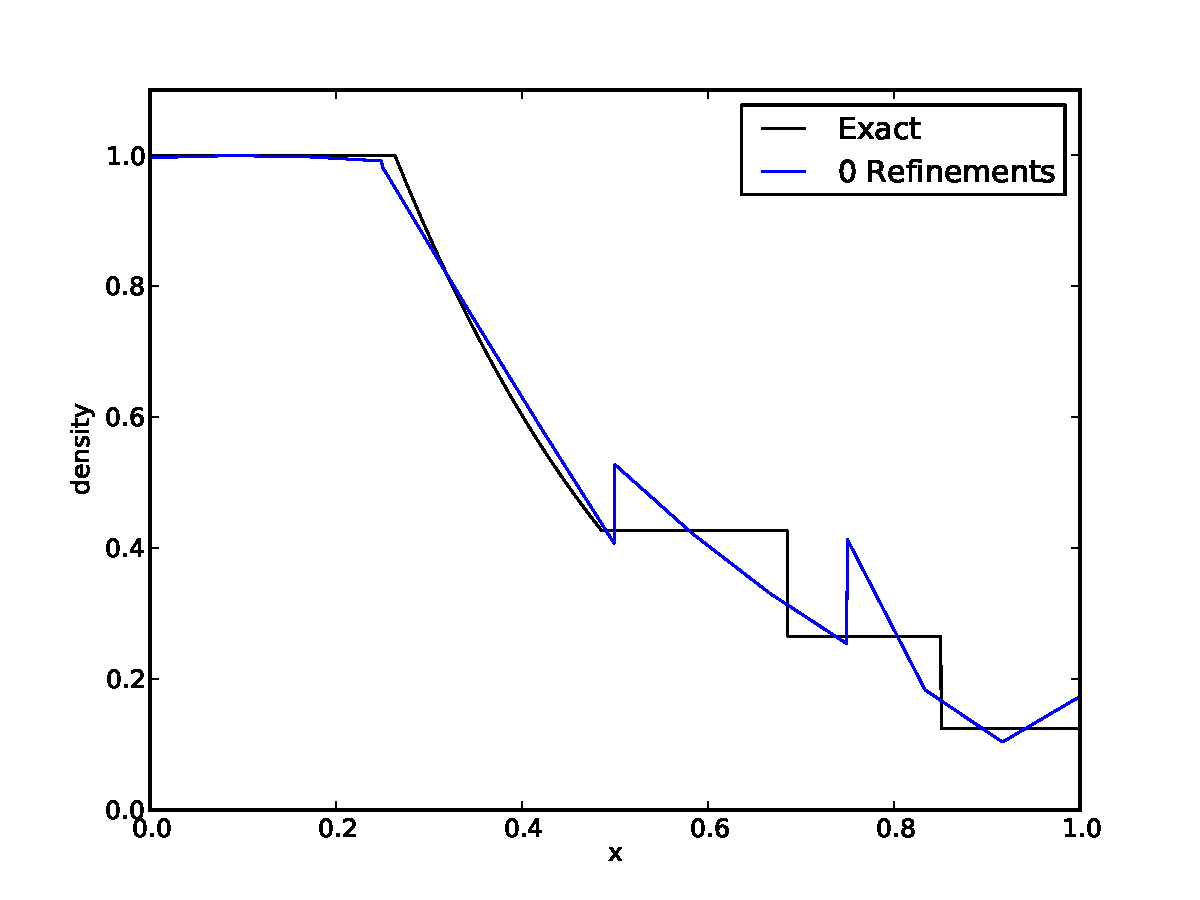
\includegraphics[width=\textwidth]{Dissertation/Sod/Robust-den1.pdf}
\caption{Density}
\end{subfigure}
\begin{subfigure}[t]{0.45\textwidth}
\centering
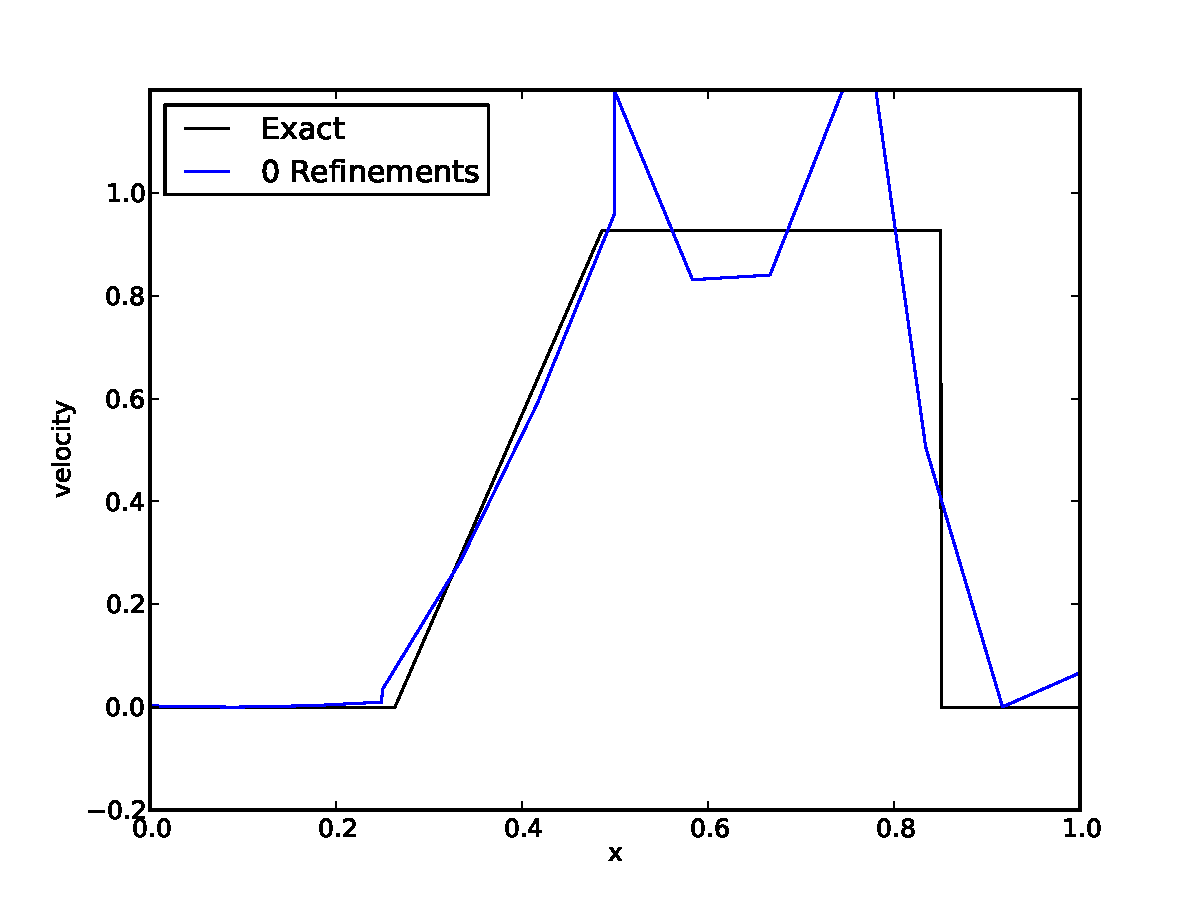
\includegraphics[width=\textwidth]{Dissertation/Sod/Robust-vel1.pdf}
\caption{Velocity}
\end{subfigure}
\begin{subfigure}[t]{0.45\textwidth}
\centering
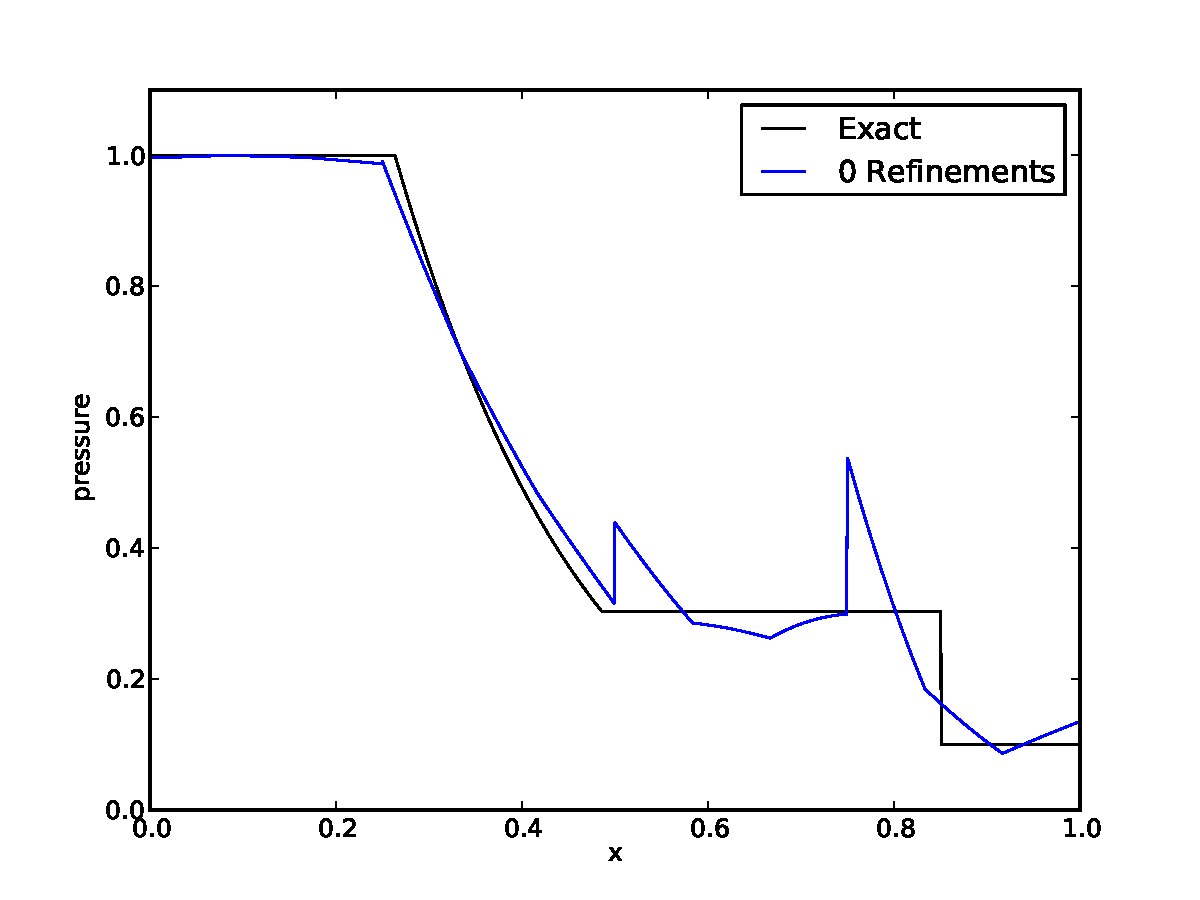
\includegraphics[width=\textwidth]{Dissertation/Sod/Robust-pres1.pdf}
\caption{Pressure}
\end{subfigure}
\begin{subfigure}[t]{\textwidth}
\centering

\includegraphics[width=\textwidth]{Dissertation/Sod/Robust-mesh1.png}
\caption{Mesh}
\end{subfigure}
\caption{Sod solution with robust norm, initial mesh}
\label{fig:SodRobust0}
\end{figure}

\begin{figure}[ht]
\centering
\begin{subfigure}[t]{0.8\textwidth}
\centering
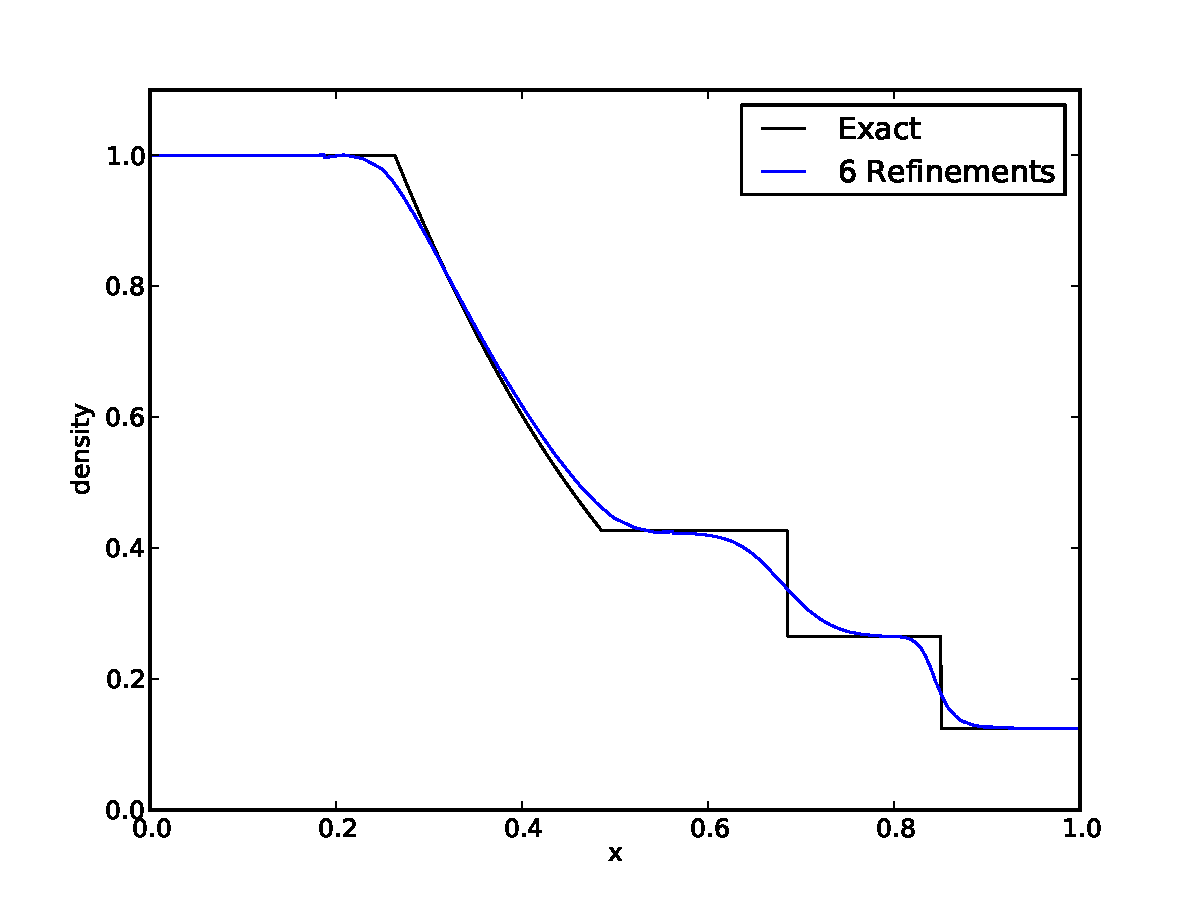
\includegraphics[width=\textwidth]{Dissertation/Sod/Robust-den7.pdf}
\caption{Density}
\end{subfigure}
\begin{subfigure}[t]{0.45\textwidth}
\centering
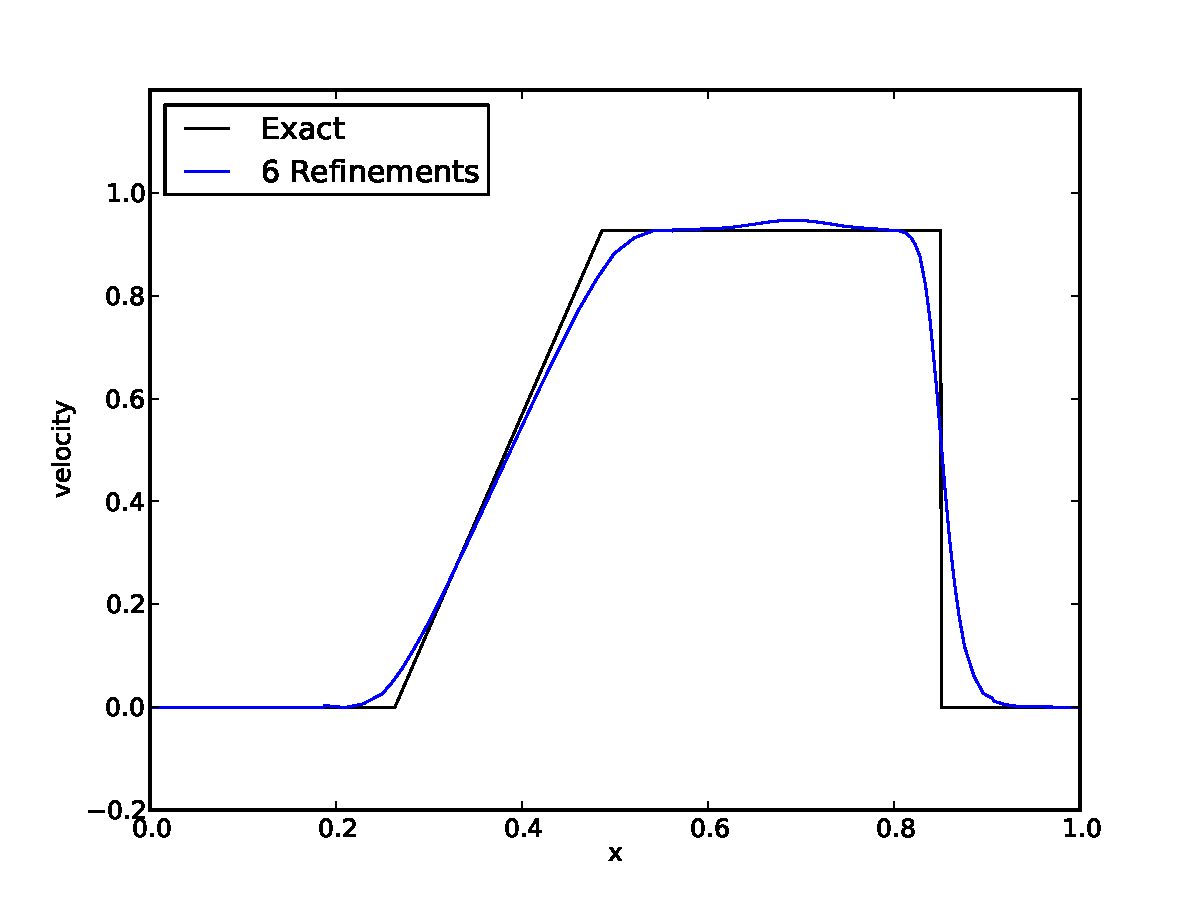
\includegraphics[width=\textwidth]{Dissertation/Sod/Robust-vel7.pdf}
\caption{Velocity}
\end{subfigure}
\begin{subfigure}[t]{0.45\textwidth}
\centering
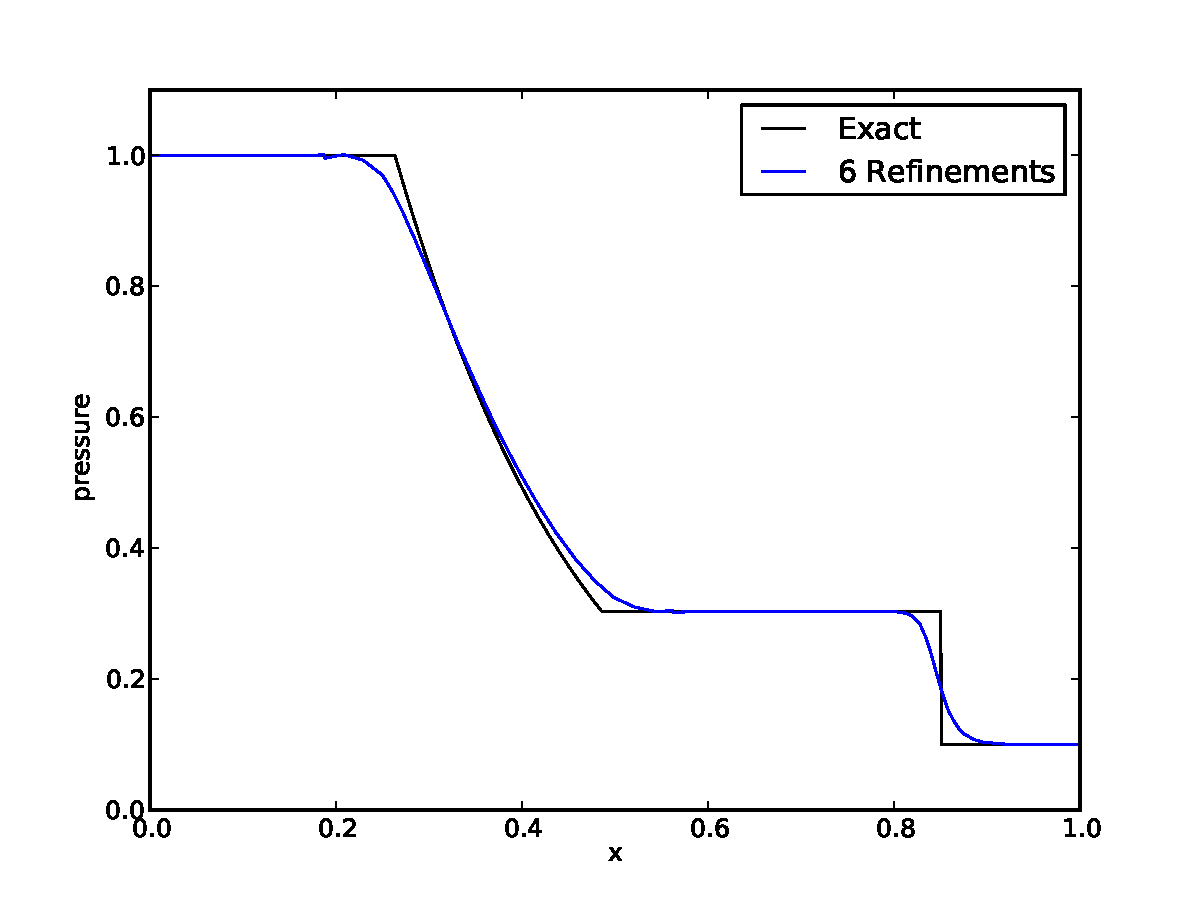
\includegraphics[width=\textwidth]{Dissertation/Sod/Robust-pres7.pdf}
\caption{Pressure}
\end{subfigure}
\begin{subfigure}[t]{\textwidth}
\centering
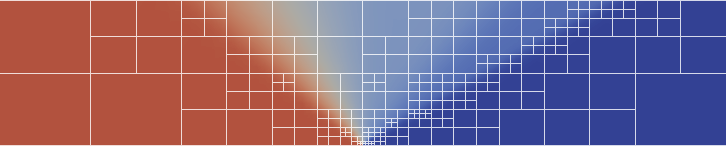
\includegraphics[width=\textwidth]{Dissertation/Sod/Robust-mesh7.png}
\caption{Mesh}
\end{subfigure}
\caption{Sod solution with robust norm, 6th refinement}
\label{fig:SodRobust6}
\end{figure}

\begin{figure}[ht]
\centering
\begin{subfigure}[t]{0.8\textwidth}
\centering
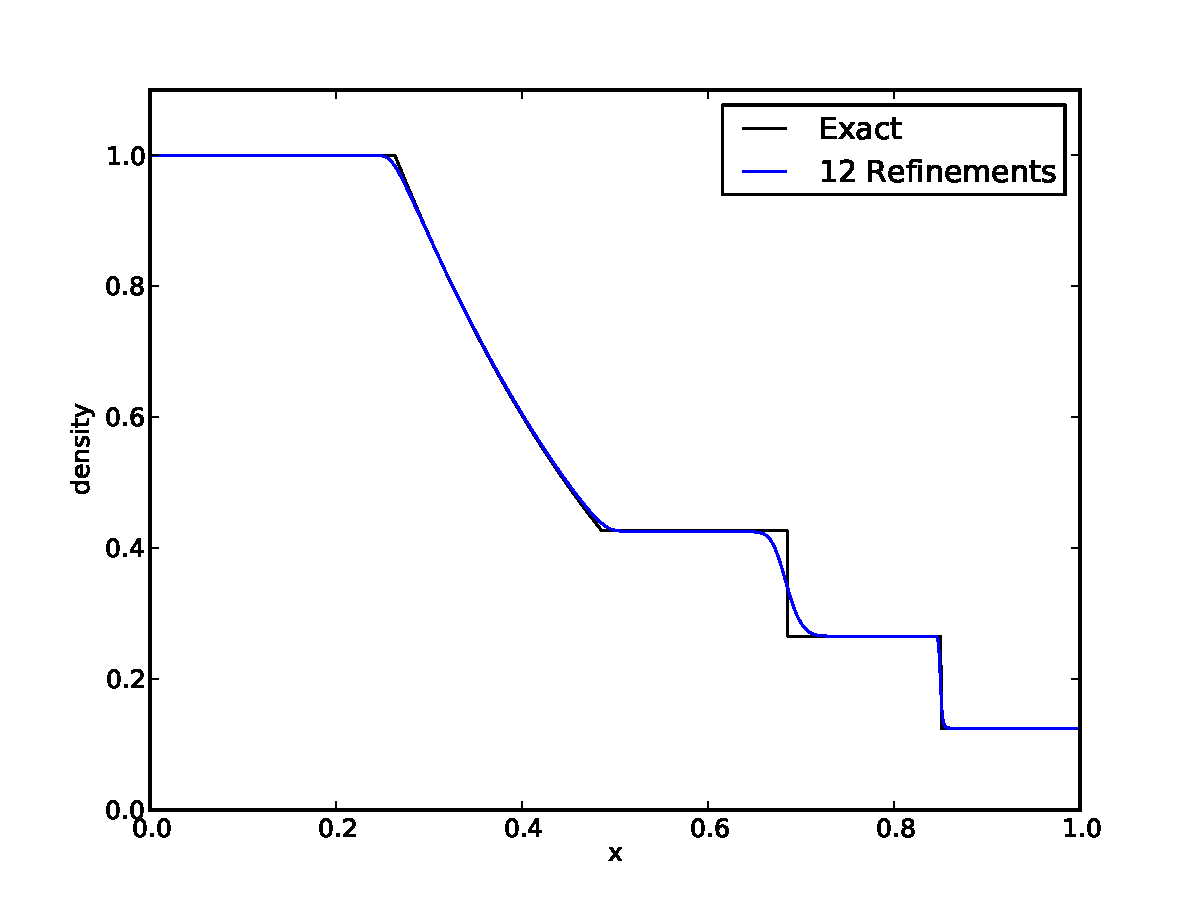
\includegraphics[width=\textwidth]{Dissertation/Sod/Robust-den13.pdf}
\caption{Density}
\end{subfigure}
\begin{subfigure}[t]{0.45\textwidth}
\centering
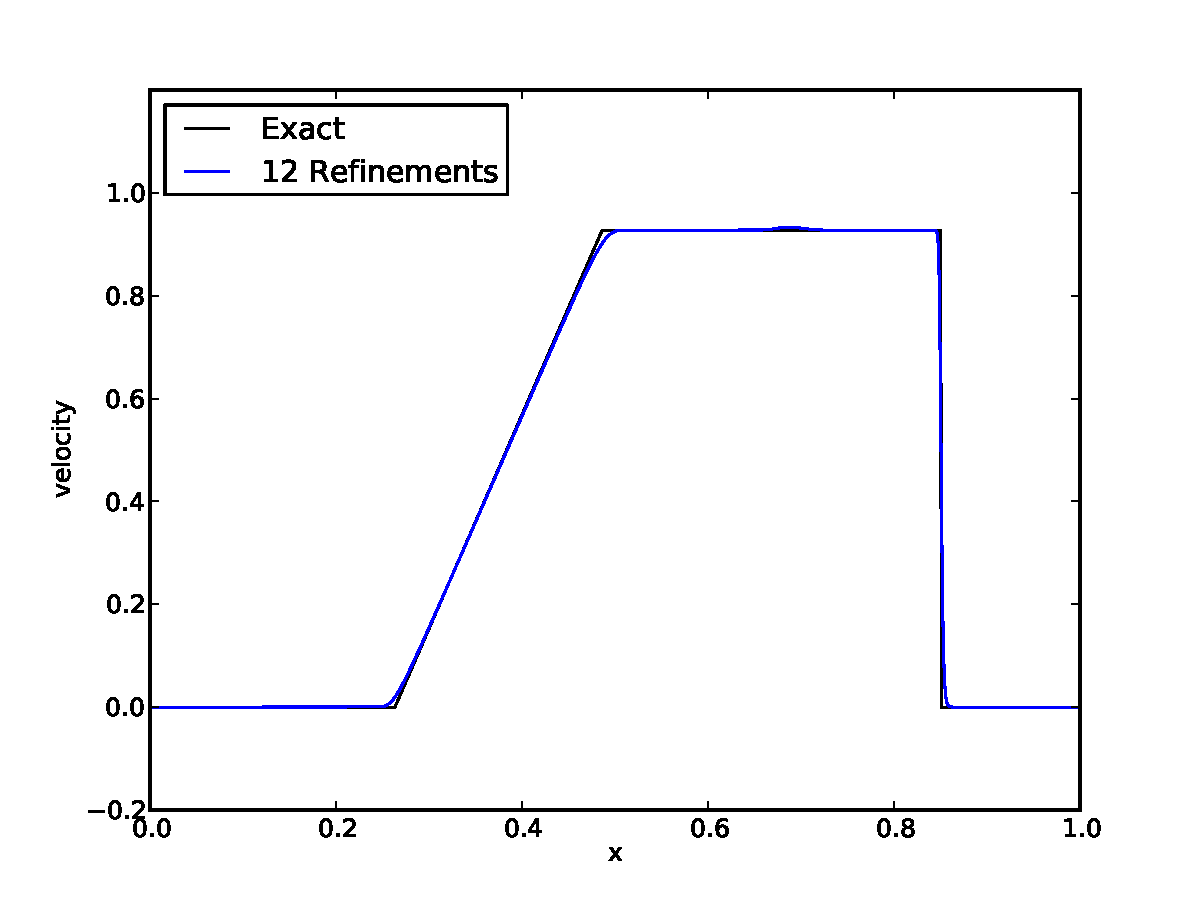
\includegraphics[width=\textwidth]{Dissertation/Sod/Robust-vel13.pdf}
\caption{Velocity}
\end{subfigure}
\begin{subfigure}[t]{0.45\textwidth}
\centering
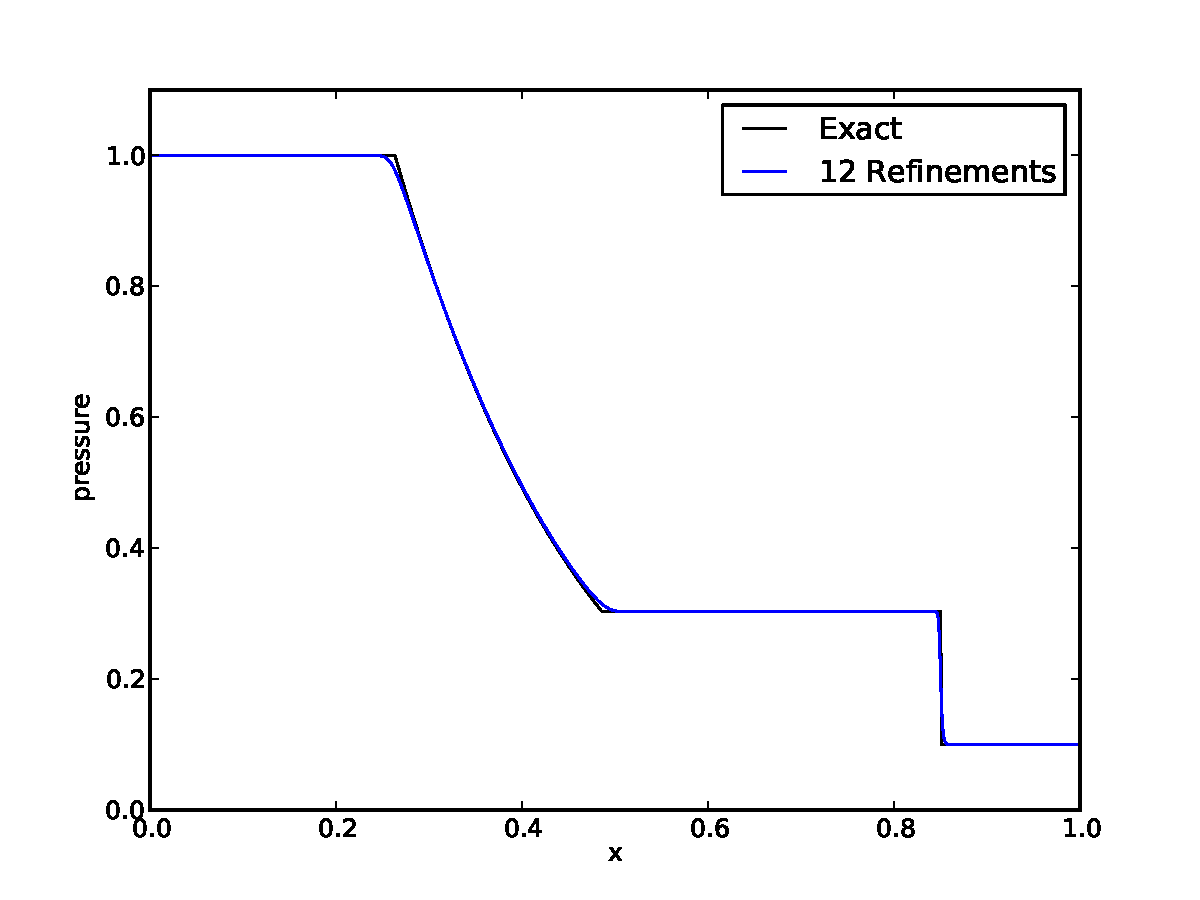
\includegraphics[width=\textwidth]{Dissertation/Sod/Robust-pres13.pdf}
\caption{Pressure}
\end{subfigure}
\begin{subfigure}[t]{\textwidth}
\centering
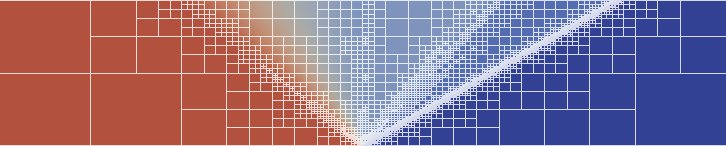
\includegraphics[width=\textwidth]{Dissertation/Sod/Robust-mesh13.png}
\caption{Mesh}
\end{subfigure}
\caption{Sod solution with robust norm, 12th refinement}
\label{fig:SodRobust12}
\end{figure}

\subsection{Noh Implosion}
% Re=1e3, p=1, delta_p=2, nlMaxIters=10, coarseRe=10
The Noh implosion problem\cite{Noh1987} is another standard test for Euler solvers.
The initial conditions are of an ideal gas with $\gamma=5/3$, zero pressure, uniform initial density of 1, 
and uniform velocity toward the center of the domain.
An infinitely strong shock propagates outward at a speed of 1/3.
For 1D flow, the post shock density jumps to 4.
The domain is $[-1,0]\times[0,1]$.
We apply boundary conditions $\hat t_c=\hat t_m=-1$, $\hat t_e=0$ on the left boundary,
symmetry conditions $\hat u=\hat t_c=\hat t_e=0$ on the right boundary, and flux conditions on $t=0$
according to the initial conditions.
We solve with $p=1$, $\Delta p=2$, $\mu_\text{fine}=10^3$, $\mu_\text{coarse}=10$, and $k=0$.
The continuation in viscosity strategy makes a significant difference keeping
the refinement pattern clean on this problem. 
If we jump straight to the final viscosity, we get a lot of spurious shock behavior on coarse meshes
which eventually go away, but leave a lot of unnecessary refinements.

The results for the initial mesh, an intermediate mesh, and the final mesh are plotted 
in Figure \ref{fig:NohRobust}. 
We see an unnecessary refinement pattern that appears in the 10th refinement mesh.
We hypothesize that this might be related to poor resolution of the error representation function
in these parts of the domain.
One notable feature of the final solution is that we don't see a drop in the density near the symmetry boundary.
This phenomena is known as wall heating and, though unphysical, appears to be nearly 
universal in simulations of this problem.
We don't perfectly match the solution, there are some wiggles at the shock front that could be resolved
better, but the fact that we don't see any noticeable wall heating is significant.


\begin{figure}[ht]
\centering
\begin{subfigure}[t]{0.32\textwidth}
\centering
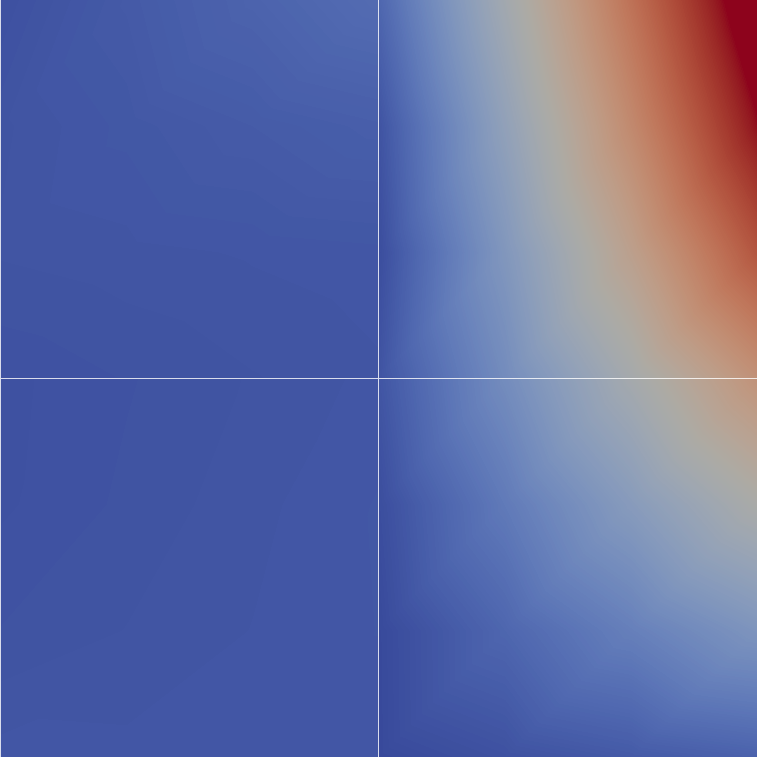
\includegraphics[width=\textwidth]{Dissertation/Noh/Robust-mesh0.png}
\caption{Initial Mesh}
\end{subfigure}
\begin{subfigure}[t]{0.32\textwidth}
\centering
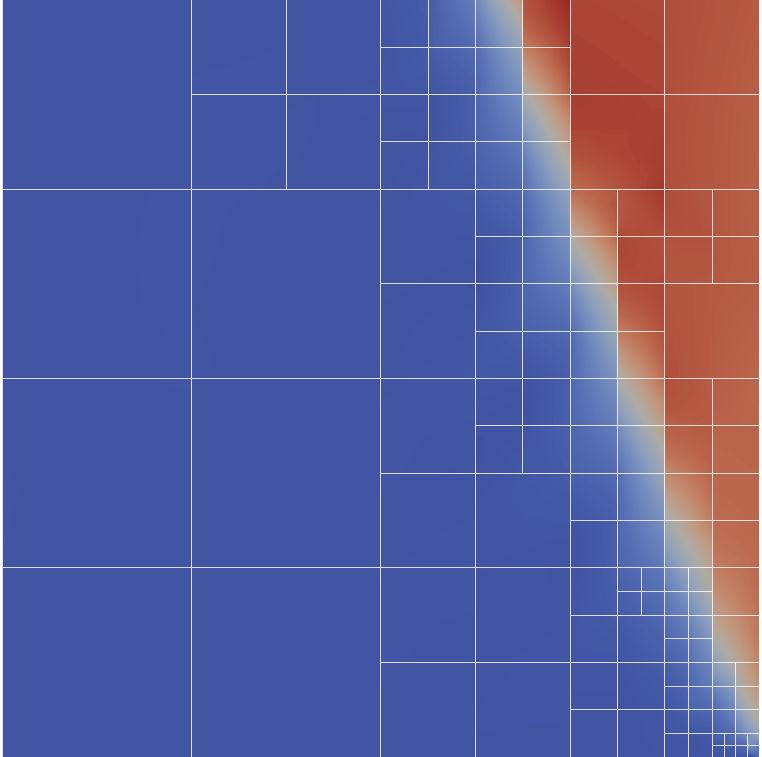
\includegraphics[width=\textwidth]{Dissertation/Noh/Robust-mesh5.png}
\caption{After 5 refinements}
\end{subfigure}
\begin{subfigure}[t]{0.32\textwidth}
\centering
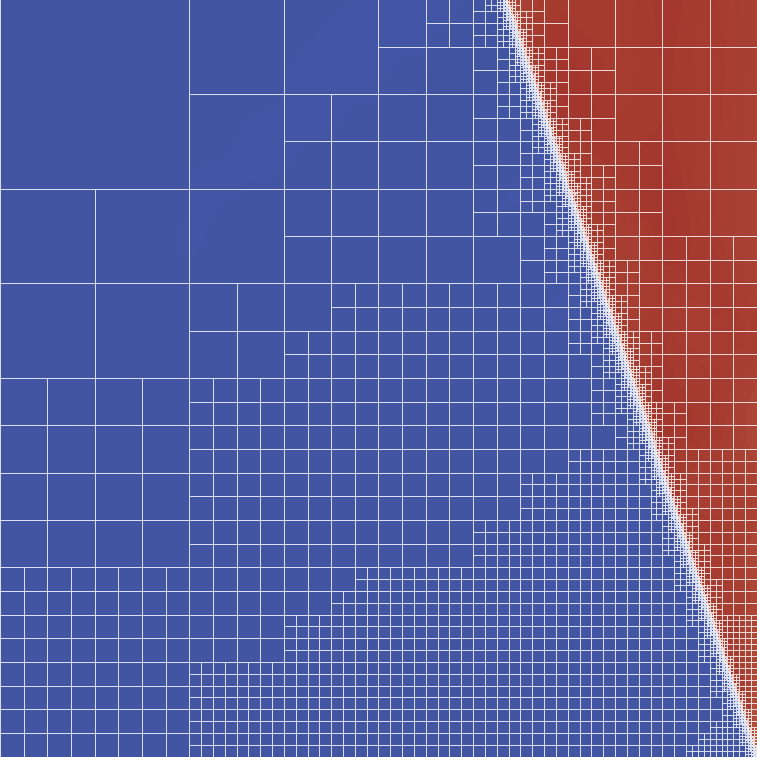
\includegraphics[width=\textwidth]{Dissertation/Noh/Robust-mesh10.png}
\caption{After 10 refinements}
\end{subfigure}
\begin{subfigure}[t]{0.9\textwidth}
\centering
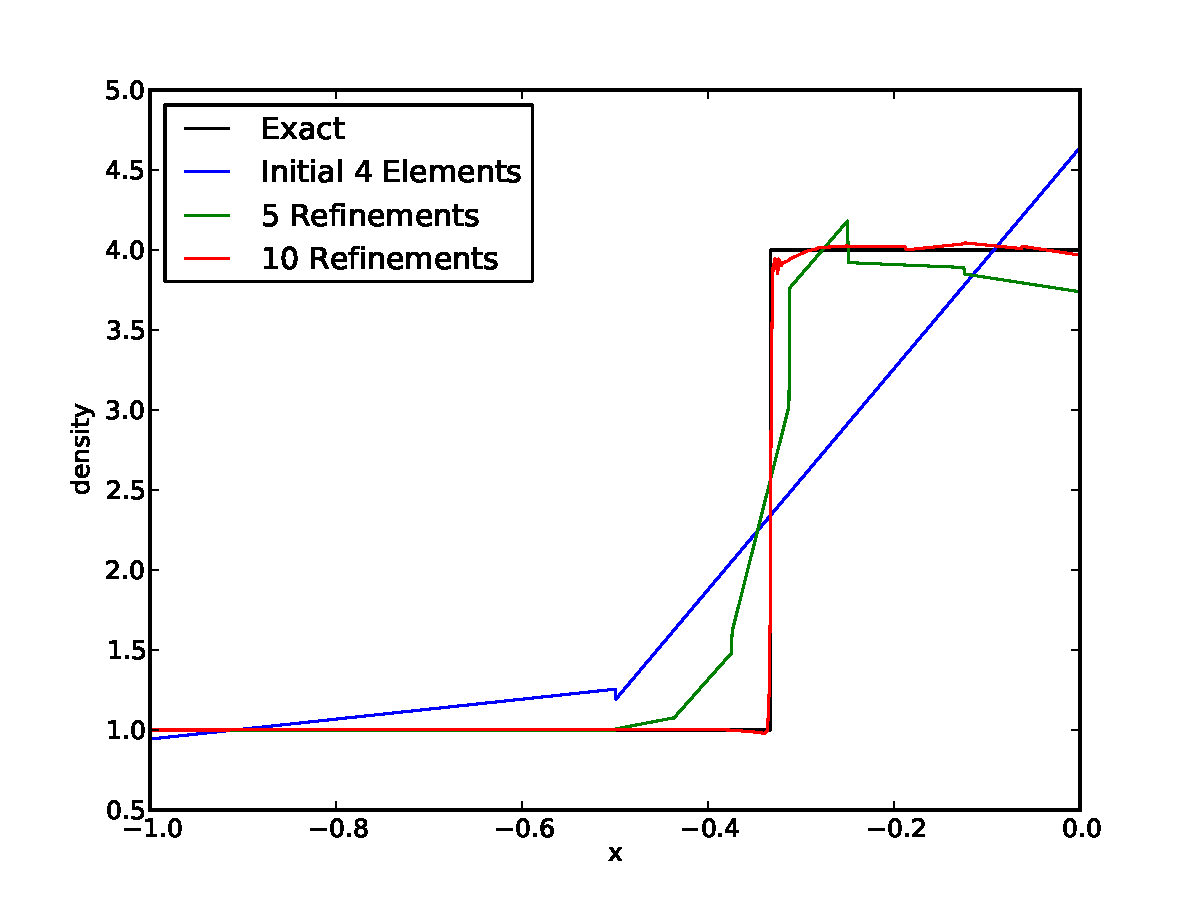
\includegraphics[width=\textwidth]{Dissertation/Noh/Robust-den.pdf}
\caption{Density at final time}
\end{subfigure}
\caption{Noh solution with robust norm}
\label{fig:NohRobust}
\end{figure}

\subsection{Piston Problem}
\label{sec:piston}
% Lesoinne and Farhat\cite{GCL} found that space-time methods provided the best satisfaction of
% geometric conservation laws for moving mesh problems compared to several other techniques. 
In the piston problem, we have a compressible gas with $\gamma=5/3$ initially at rest with zero pressure.
At $t=0$, the left wall of the domain (initially $[0,1]$) starts moving inward at a velocity of 1.
This triggers a shock which precedes the moving piston and collides with the stationary right wall 
at $t=0.8$. The initial density is 1, but jumps to 4 after the first shock, and 10 after the second.
By the final time of $t=0.85$ the second shock has traversed half the remaining distance from
the right wall to the piston.
The symmetry conditions from the Noh problem are applied on the right wall. 
The left boundary has normal $n_{xt}=(-\sqrt{2},\sqrt{2})$ which means that fluxes at our disposal are:
\begin{align*}
\hat t_c&=\sqrt{2}(-\rho u+\rho)\\
\hat t_m&=\sqrt{2}(-\rho u^2-\rho RT+\rho u)\\
\hat t_e&=\sqrt{2}(-\rho u(C_vT+\frac{1}{2}u^2)-u\rho RT+\rho(C_vT+\frac{1}{2}u^2))\,,
\end{align*}
and since $u=1$ at the left wall
\begin{align*}
\hat t_c&=0\\
\hat t_m&=-\sqrt{2}\rho RT\\
\hat t_e&=-\sqrt{2}\rho RT\,.
\end{align*}
Therefore we set the following boundary conditions at the left boundary: $\hat u=1$, $\hat t_c=0$, 
and $\hat t_m-\hat t_e=0$ implemented as a penalty condition.
We solve using $p=2$, $\Delta p=2$, a fixed $\mu=100$, and an initial $4\times4$ space-time mesh.
Unfortunately, the robust and coupled robust norms did not produce the cleanest solutions
on this problem, and we were forced to use the NSDecoupled norm which has
less mathematical justification but seems to work very well on shock problems.
Final results and mesh are shown in Figure~\ref{fig:PistonSolution} and Figure~\ref{fig:PistonMesh}.

\begin{figure}[ht]
\centering
\begin{subfigure}[t]{0.7\textwidth}
\centering
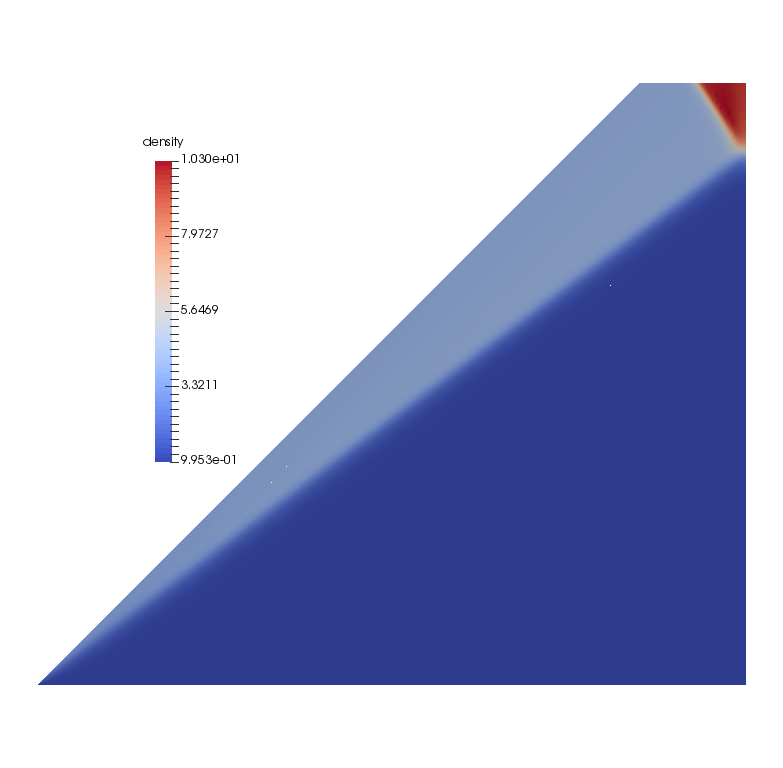
\includegraphics[width=\textwidth]{Piston/Piston_density.png}
\caption{Density}
\end{subfigure}
\begin{subfigure}[t]{0.7\textwidth}
\centering
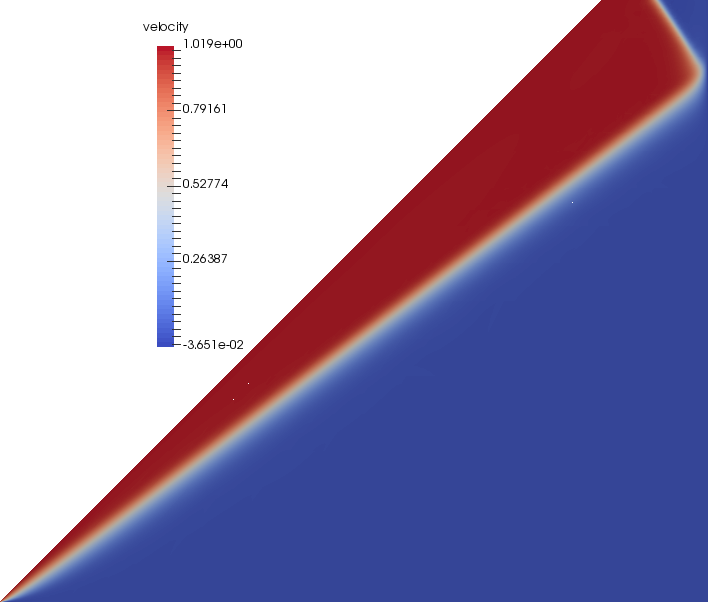
\includegraphics[width=\textwidth]{Piston/Piston_velocity.png}
\caption{Velocity}
\end{subfigure}
% \begin{subfigure}[t]{0.45\textwidth}
% \centering
% 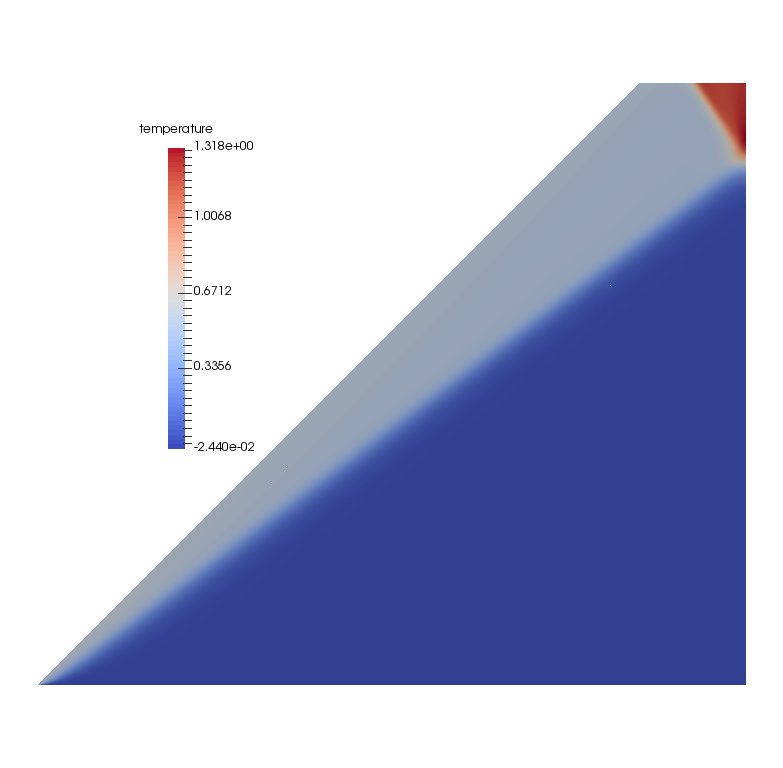
\includegraphics[width=\textwidth]{Piston/Piston_temp.png}
% \caption{Temperature}
% \end{subfigure}
% \begin{subfigure}[t]{0.7\textwidth}
% \centering
% 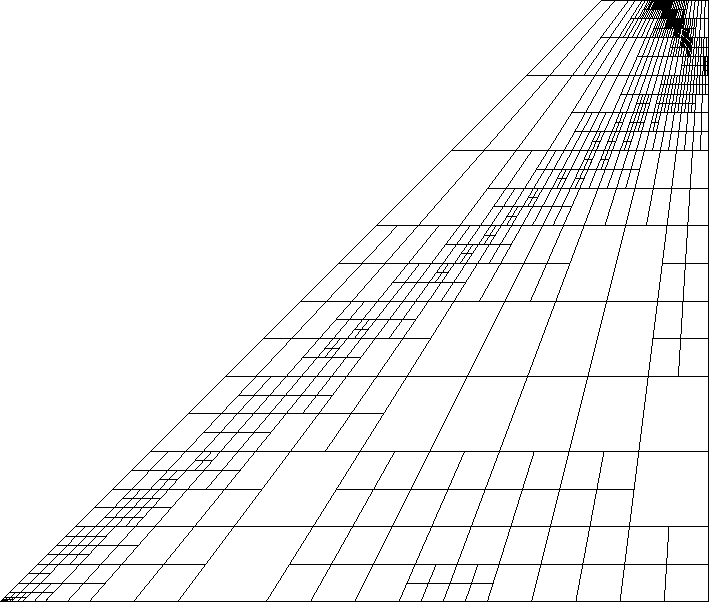
\includegraphics[width=\textwidth]{Piston/Piston_mesh.png}
% \caption{Mesh}
% \end{subfigure}
\caption{Piston solution with NSDecoupled norm after 8 adaptive refinements}
\label{fig:PistonSolution}
\end{figure}

\begin{figure}[ht]
\centering
% \begin{subfigure}[t]{0.7\textwidth}
% \centering
% 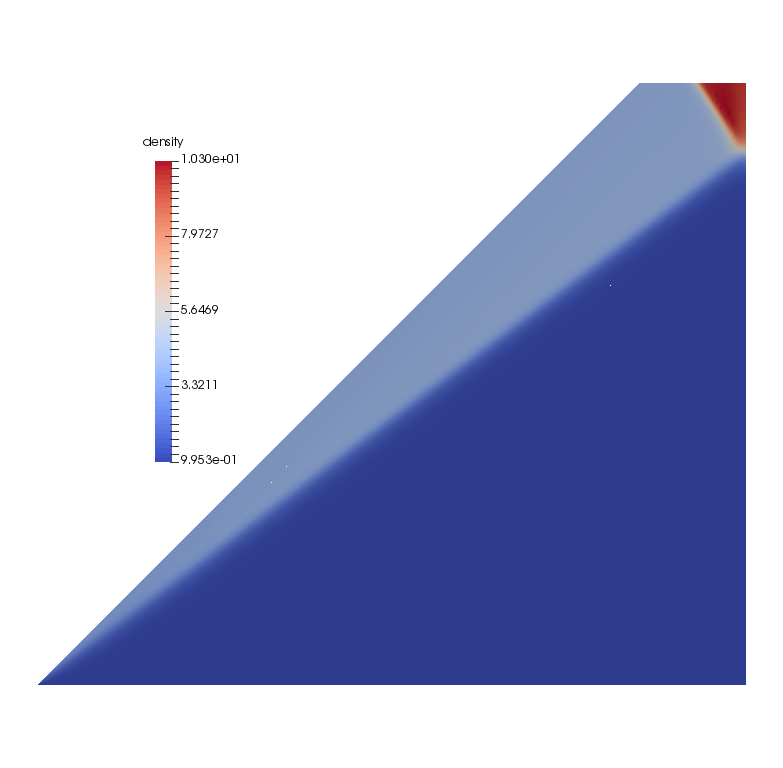
\includegraphics[width=\textwidth]{Piston/Piston_density.png}
% \caption{Density}
% \end{subfigure}
% \begin{subfigure}[t]{0.45\textwidth}
% \centering
% 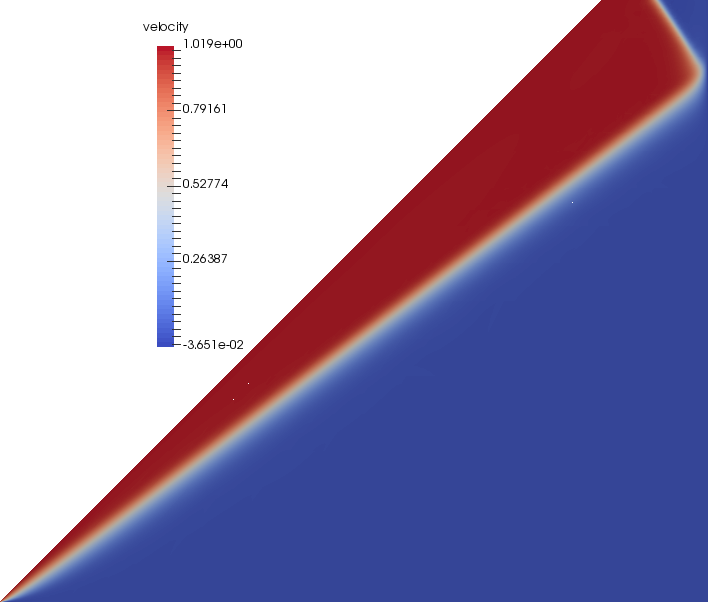
\includegraphics[width=\textwidth]{Piston/Piston_velocity.png}
% \caption{Velocity}
% \end{subfigure}
% \begin{subfigure}[t]{0.45\textwidth}
% \centering
% 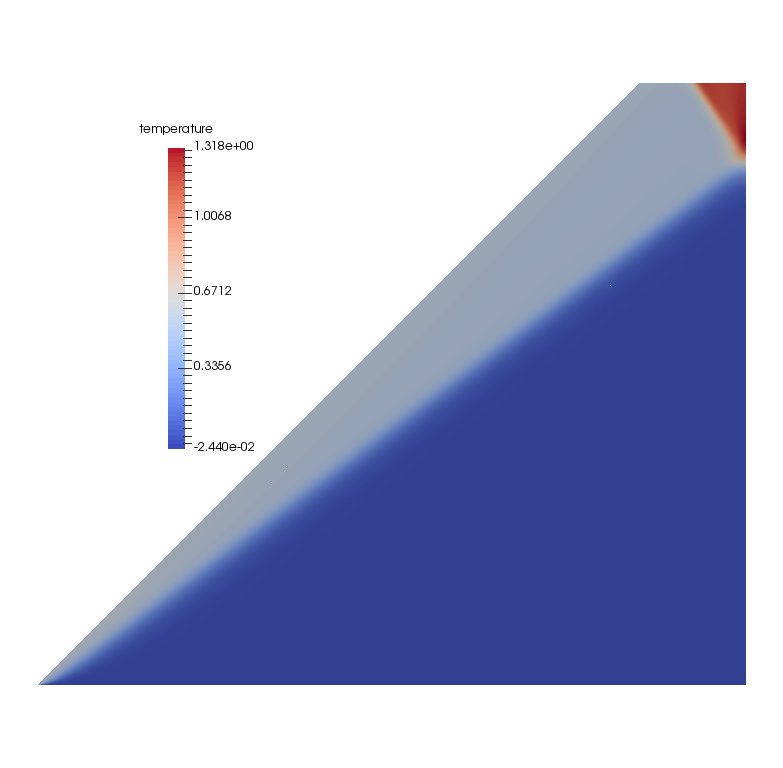
\includegraphics[width=\textwidth]{Piston/Piston_temp.png}
% \caption{Temperature}
% \end{subfigure}
% \begin{subfigure}[t]{0.7\textwidth}
\centering
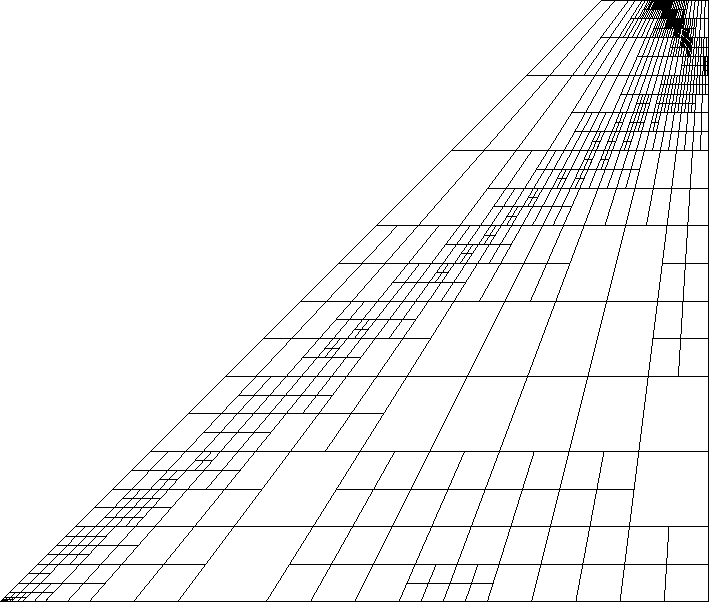
\includegraphics[width=\textwidth]{Piston/Piston_mesh.png}
% \caption{Mesh}
% \end{subfigure}
\caption{Piston mesh with NSDecoupled norm after 8 adaptive refinements}
\label{fig:PistonMesh}
\end{figure}

% \textcolor{red}{\subsection{Possible 2D Results}
% Attempting the following
% \begin{enumerate}
% \item{Noh}
% \item{Compressible Taylor-Green}
% \item{Sedov}
% \item{Triple Point}
% \item{Rayleigh-Taylor Instability}
% \end{enumerate}
% }

\section{Summary of Compressible Results}
The chief strength of the DPG method is in its stability and adaptivity properties.
It makes no claims of being a robust technique for handling shocks
and in fact we ran into a lot of shock related difficulties in arriving at these solutions.
The continuation in viscosity strategy, though avoidable, was an attempt at mitigating these challenges.
What is notable is that we were able to initialize each simulation from very coarse meshes
and adaptively resolve the solution features.

\end{document}
